\title{EE382V Multicore Computing: Assignment 1} 

\author{
		Wenwen Zhang [wz3585]\\        
        Chunheng Luo [cl38532]\\
}

\date{\today}

\documentclass[12pt]{article}
\setlength{\parindent}{0em} 
\setlength{\parskip}{1em}
\renewcommand{\baselinestretch}{1.0} 
\usepackage{listings}
\usepackage{color}
\usepackage{enumitem}
\usepackage{amsmath}
\usepackage{graphicx}

\lstset{basicstyle=\footnotesize\ttfamily,breaklines=true}

\begin{document}
\maketitle

\section*{Question 0} 
TACC User IDs:
\begin{itemize}
\vspace{-1ex}
\item Wenwen Zhang: wenwen22  \\
\vspace{-1ex}
\item Chunheng Luo: chluo     \\
\vspace{-1ex}
\end{itemize}

\section*{Question 1}

\textbf{Part (a)}

\begin{itemize} 
\item Assuming other parts of the program can be sped up by the factor of $n$, then the overall speedup is $$Speedup = \dfrac{1}{0.4+\dfrac{0.6}{n}}$$  \\
\item Assuming the method M accounts for $x$ of the program's execution time on a single-core processor, M can be sped up by $2^3$ and other parts of the program can be sped up by the factor of $n$, then the overall speedup is $$Speedup = \dfrac{1}{\dfrac{x}{8} + \dfrac{(1-x)}{n}}$$
So in order to double the speedup, we require $$\dfrac{1}{ \dfrac{x}{8} + \dfrac{(1-x)}{n}} = 2\times\dfrac{1}{0.4+\dfrac{0.6}{n}}$$ 
which leads to $$x = \dfrac{0.2n - 0.7}{0.125n - 1}$$ \\
Therefore, M must account for $(0.2n - 0.7)/(0.125n - 1)$ of the total execution time \textbf{on a single-core processor} in order to double the overall speedup of the program. 
\end{itemize}

\textbf{Part (b)} \\ 

Assuming the parts of the program that can be totally parallelized account for $P$ of the total execution time on a single-core processor, and all of the other parts of the program, which accounts for $(1-P)$ of the total execution time on a single-core processor, are not able to gain any speedup from the multicore architecture, then we have 
$$S_2 = \dfrac{1}{(1-P) + \dfrac{P}{2}}$$ and $$S_n = \dfrac{1}{(1-P) + \dfrac{P}{n}}$$
Solving the equations, we get $$S_n = \dfrac{nS_2}{(2-n)S_2 + 2(n-1)}$$ 

\section*{Question 2}

\section*{Question 3} 
In order make Filter Algorithm able to solve the l-exclusion problem, we can simply reduce the number gates from $N$ to $(N - l)$. \\
\noindent\rule[0.5ex]{\linewidth}{1pt}
\begin{lstlisting}[language=C] 
const int  N;           
int[N]     gate init 0; 
int[N-l+1] last init 0; 

/* For P_i */ 
request CS; 
for (k = 1 : N - l) { 
  gate[i] = k;          // P_i is at gate k 
  last[k] = i;          // P_i updates last for that gate 
	
  int numAhead = l + 1;   
  while (numAhead > l && last[k] == i) {
    for (j = 1 : N - 1) {
	  if (j != i && gate[j] >= k) 
	    numAhead += 1; 
    }
  }
}
CS; 
release CS; 
gate[i] = 0; 
\end{lstlisting}
\noindent\rule[0.5ex]{\linewidth}{1pt}

\section*{Question 4} 
* Code submitted on Canvas. 

\section*{Question 5}  
* Code submitted on Canvas. The execution time plot is shown in Fig 1. 
\begin{figure} 
	 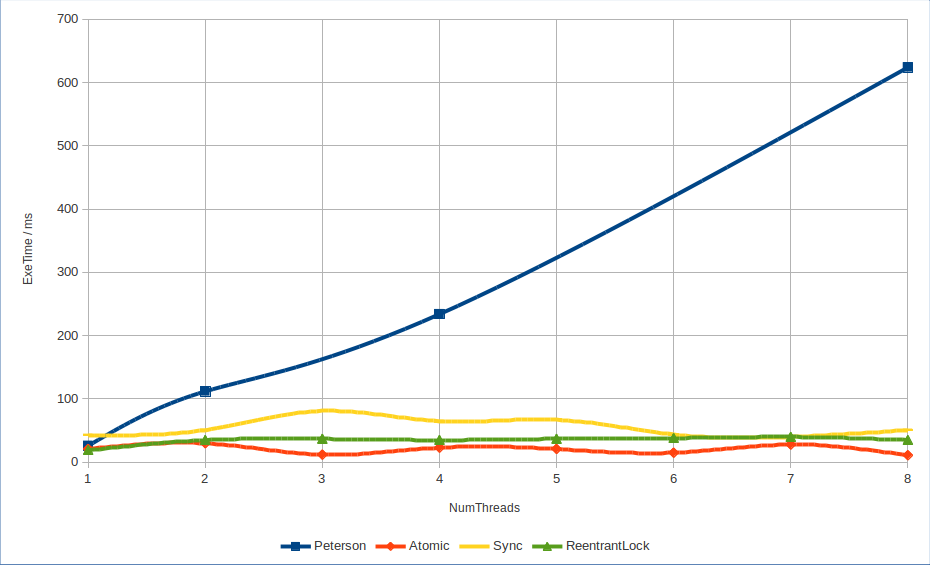
\includegraphics[width=\linewidth]{plot.png}
	 \caption{Execution time using the four methods}
\end{figure} 


\end{document}
